
\subsection{推定値の合成(Estimator Fusion)}
$f(\theta,x)=\phi(x)\theta$ の線形回帰で,$D_N$ と $D'_M$ から得た推定
\(
\hat\theta_N=\Phi_N \sum_{i=1}^N \phi_i^\top y_i,\;
\hat\theta'_M=\Phi'_M \sum_{j=1}^M \phi'_j{}^\top y'_j
\)
($\Phi_N=(\sum \phi_i^\top\phi_i)^{-1}$)を持つとき,結合推定は
\[
  \hat\theta_{N+M}
  =\bigl(\Phi_N^{-1}+\Phi_M'{}^{-1}\bigr)^{-1}
   \bigl(\Phi_N^{-1}\hat\theta_N+\Phi_M'{}^{-1}\hat\theta'_M\bigr)
\]
で与えられる。\cite{exp2025}

\paragraph{実装例(R)}
\begin{lstlisting}
# 既存バッチN=6000とM=4000の合成(S = Φ^{-1} を情報行列とする)
# S_6000, S_4000 はそれぞれ Φ_6000^{-1}, Φ_4000^{-1}
# theta_6000, theta_4000 は各バッチの推定ベクトル
theta_6000_4000 <- solve(S_6000 + S_4000) %*%
  (S_6000 %*% theta_6000 + S_4000 %*% theta_4000)
\end{lstlisting}

\subsection{逐次最小二乗法(RLS)}
逆行列補題を用いると,バッチ解は次の再帰で更新できる:
\[
\begin{aligned}
  \hat\theta_{N+1} &= \hat\theta_N + K_{N+1}\bigl(y_{N+1}-\phi_{N+1}\hat\theta_N\bigr),\\
  K_{N+1} &= \Phi_N \phi_{N+1}^\top\bigl(I_m + \phi_{N+1}\Phi_N\phi_{N+1}^\top\bigr)^{-1},\\
  \Phi_{N+1} &= \Phi_N - K_{N+1}\phi_{N+1}\Phi_N .
\end{aligned}
\]
忘却係数 $\gamma\in(0,1]$ を導入すると
\[
\begin{aligned}
  K_{\gamma,N+1} &= \Phi_{\gamma,N}\phi_{N+1}^\top
    \bigl(\gamma I_m+\phi_{N+1}\Phi_{\gamma,N}\phi_{N+1}^\top\bigr)^{-1},\\
  \Phi_{\gamma,N+1} &= \gamma^{-1}\!\left(\Phi_{\gamma,N}-K_{\gamma,N+1}\phi_{N+1}\Phi_{\gamma,N}\right),\\
  \hat\theta_{\gamma,N+1} &= \hat\theta_{\gamma,N} +
    K_{\gamma,N+1}\bigl(y_{N+1}-\phi_{N+1}\hat\theta_{\gamma,N}\bigr).
\end{aligned}
\]
\cite{exp2025}

\paragraph{実装例(R,忘却係数つき更新関数)}
\begin{lstlisting}
update_regression_mat <- function(Phi_N, phi_N_plus_1, theta_N, y_N_plus_1, gamma = 1){
  I_m <- diag(1)  # m=1想定。m>1なら diag(nrow(phi_N_plus_1 %*% Phi_N %*% t(phi_N_plus_1))) に置換
  # 中間計算
  phi_T_Phi_phi <- phi_N_plus_1 %*% Phi_N %*% t(phi_N_plus_1)
  inv_term <- solve( (gamma * I_m) + phi_T_Phi_phi )
  K <- gamma * (Phi_N %*% t(phi_N_plus_1) %*% inv_term)
  # 更新
  Phi_N_plus_1 <- (Phi_N - K %*% phi_N_plus_1 %*% Phi_N ) / gamma
  theta_N_plus_1 <- theta_N + K %*% (y_N_plus_1 - phi_N_plus_1 %*% theta_N)
  list(Phi_N_plus_1 = Phi_N_plus_1, theta_N_plus_1 = theta_N_plus_1)
}
\end{lstlisting}

\paragraph{初期化と計算量}
$\Phi_0=\varepsilon^{-1}I$(小 $\varepsilon$)で初期化し,逐次更新する。各ステップの計算は
$\dim(\theta)=p$ に対して $O(p^2)$ 程度で済む。\cite{exp2025}

\subsection{課題7(推定値の合成の検証:2分割データの統合)}

\paragraph{課題の内容}
$N=10000$ のデータを前半 $6000$ と後半 $4000$ に分割し,各ブロックで OLS 推定を行ったのち,情報行列の加法性
\[
  S_N \;=\; \sum_{i=1}^N \varphi_i \varphi_i^\top
\]
を用いた合成推定
\[
  \hat\theta_{\mathrm{fuse}}
  \;=\;
  \bigl(S_{6000}+S_{4000}\bigr)^{-1}
  \Bigl(S_{6000}\hat\theta_{6000}+S_{4000}\hat\theta_{4000}\Bigr)
\]
が,全データ一括推定 $\hat\theta_{10000}$ と一致することを確認する。ここでモデルは
\[
  y_i \;=\; \varphi(x_i)^\top \theta + w_i,\quad
  \varphi(x)=
  \begin{bmatrix}
    1\\[1mm]
    \exp\!\bigl(-\tfrac{(x-1)^2}{2}\bigr)\\[1mm]
    \exp\!\bigl(-(x+1)^2\bigr)
  \end{bmatrix}\!,
\quad \theta\in\mathbb{R}^3.
\]
理論上,独立同分布で $V=\sigma^2$ のとき $\hat\theta_{\mathrm{fuse}}=\hat\theta_{10000}$ となる。\cite{exp2025}

\paragraph{実装}
分割データから
\(
S_{6000},\hat\theta_{6000},\;S_{4000},\hat\theta_{4000}
\)
を得て,合成推定値を計算し,全データ一括推定と比較する。

\begin{lstlisting}
# 事前に x, y, x_6000, y_6000, x_4000, y_4000 を用意済み

exp7 <- function(){
  res6000 <- regression_multiple(x_6000, y_6000)
  res4000 <- regression_multiple(x_4000, y_4000)
  res10000 <- regression_multiple(x, y)

  S_6000 <- res6000$S
  S_4000 <- res4000$S
  theta_6000 <- res6000$theta_hat
  theta_4000 <- res4000$theta_hat

  # 推定値の合成(情報行列の和)
  theta_6000_4000 <- solve(S_6000 + S_4000) %*%
    (S_6000 %*% theta_6000 + S_4000 %*% theta_4000)

  cat("S6000:\n"); print(S_6000)
  cat("S4000:\n"); print(S_4000)
  cat("theta6000:\n"); print(theta_6000)
  cat("theta4000:\n"); print(theta_4000)
  cat("theta_fuse:\n"); print(theta_6000_4000)

  theta_10000 <- res10000$theta_hat
  cat("theta10000:\n"); print(theta_10000)

  # 一致性の確認(数値誤差内)
  cat("all.equal(theta_fuse, theta10000): ",
      all.equal(drop(theta_6000_4000), drop(theta_10000),
                tolerance = 1e-10), "\n")
}

exp7()
\end{lstlisting}

\paragraph{結果}
一例として,実行時に次を得た。
\[
S_{6000}=
\begin{bmatrix}
6000.000 & 1505.370 & 1033.499\\
1505.370 & 1063.211 & 226.401\\
1033.499 & 226.401 & 720.562
\end{bmatrix},\quad
S_{4000}=
\begin{bmatrix}
4000.000 & 971.151 & 716.318\\
971.151 & 679.477 & 149.749\\
716.318 & 149.749 & 510.224
\end{bmatrix},
\]
\[
\hat\theta_{6000}=
\begin{bmatrix}
-0.003879385\\ 3.010714895\\ -1.989434350
\end{bmatrix},\;
\hat\theta_{4000}=
\begin{bmatrix}
-0.02537589\\ 3.03489937\\ -1.97772731
\end{bmatrix},\;
\hat\theta_{\mathrm{fuse}}=
\begin{bmatrix}
-0.0124955\\ 3.0204300\\ -1.9848692
\end{bmatrix}.
\]
全データ一括推定 $\hat\theta_{10000}$ と $\hat\theta_{\mathrm{fuse}}$ は数値誤差内で一致した(コードで \verb|all.equal| により検証)。

\paragraph{考察}
% (ここに考察を記述)

\subsection{課題7(推定値の合成の検証:非線形基底・分割データ)}

\paragraph{課題の内容}
基底
\[
  \varphi(x)=
  \begin{bmatrix}
    1\\[1mm]
    \exp\!\bigl(-\tfrac{(x-1)^2}{2}\bigr)\\[1mm]
    \exp\!\bigl(-(x+1)^2\bigr)
  \end{bmatrix}\!,\qquad
  y_i=\varphi(x_i)^\top \theta+w_i,\ \theta\in\mathbb{R}^3
\]
で $N=10000$ 個のデータを前半 $6000$ と後半 $4000$ に分割する。
各ブロックの推定値 $(\hat\theta_{6000},\hat\theta_{4000})$ と情報行列
$S_k=\sum_{i\in\text{block }k}\varphi_i\varphi_i^\top$ を用いて
\[
  \hat\theta_{\mathrm{fuse}}
  =(S_{6000}+S_{4000})^{-1}\!\bigl(S_{6000}\hat\theta_{6000}+S_{4000}\hat\theta_{4000}\bigr)
\]
を計算し,全データ一括推定 $\hat\theta_{10000}$ と照合する。\cite{exp2025}

\paragraph{実装(OLS 版)}
\begin{lstlisting}
data <- read.csv("datas/mmse_kadai7.csv", header=FALSE, col.names=c("x","y"))
x0 <- rep(1, nrow(data))
x1 <- exp(-(data$x - 1)^2 / 2)
x2 <- exp(-(data$x + 1)^2)
n  <- nrow(data)
x  <- array(0, dim=c(3,1,n))
for(i in 1:n){ x[,,i] <- matrix(c(x0[i], x1[i], x2[i]), 3, 1) }
y <- as.matrix(data[,"y"])

x_6000 <- x[,,1:6000, drop=FALSE]; y_6000 <- y[1:6000, , drop=FALSE]
x_4000 <- x[,,6001:10000, drop=FALSE]; y_4000 <- y[6001:10000, , drop=FALSE]

exp7 <- function(){
  r6 <- regression_multiple(x_6000, y_6000)  # returns $S$ and $theta_hat$
  r4 <- regression_multiple(x_4000, y_4000)
  rall <- regression_multiple(x, y)

  S_6000 <- r6$S;  S_4000 <- r4$S
  th6 <- r6$theta_hat; th4 <- r4$theta_hat; th_all <- rall$theta_hat

  th_fuse <- solve(S_6000 + S_4000) %*% (S_6000 %*% th6 + S_4000 %*% th4)

  print(th6); print(th4); print(th_fuse); print(th_all)
  # 一致検証
  print(all.equal(drop(th_fuse), drop(th_all), tolerance=1e-12))
}
exp7()
\end{lstlisting}

\paragraph{実装(推定分散による重み付き合成)}
各ブロックの誤差分散を
\[
  \hat\sigma_k^2=\frac{\mathrm{RSS}_k}{N_k-p},\quad p=3
\]
で推定し,$Q_k=\hat\sigma_k^{-2}$ を用いた WLS 情報行列
$S_k=\sum_{i\in k}\varphi_i Q_k \varphi_i^\top=Q_k\sum_{i\in k}\varphi_i\varphi_i^\top$
で合成する($k\in\{6000,4000\}$)。コードは次のとおり。
\begin{lstlisting}
x_mat       <- t(matrix(x,       nrow=3, ncol=n))
x_6000_mat  <- t(matrix(x_6000,  nrow=3, ncol=6000))
x_4000_mat  <- t(matrix(x_4000,  nrow=3, ncol=4000))

exp8 <- function(){
  # OLS 推定
  th_all  <- regression_multiple(x,       y)$theta_hat
  th_6000 <- regression_multiple(x_6000,  y_6000)$theta_hat
  th_4000 <- regression_multiple(x_4000,  y_4000)$theta_hat

  # 分散推定(MSE)
  V_hat_full  <- sum((y       - x_mat      %*% th_all )^2)  /(nrow(x_mat)      - ncol(x_mat))
  V_hat_6000  <- sum((y_6000  - x_6000_mat %*% th_6000)^2) /(nrow(x_6000_mat)  - ncol(x_6000_mat))
  V_hat_4000  <- sum((y_4000  - x_4000_mat %*% th_4000)^2) /(nrow(x_4000_mat)  - ncol(x_4000_mat))

  # 各ブロックの WLS 情報行列と推定
  r6 <- regression_multiple(x_6000,  y_6000, V=V_hat_6000)
  r4 <- regression_multiple(x_4000,  y_4000, V=V_hat_4000)
  S_6000 <- r6$S;  S_4000 <- r4$S
  th6 <- r6$theta_hat; th4 <- r4$theta_hat

  # 合成推定(WLS 版)
  th_fuse <- solve(S_6000 + S_4000) %*% (S_6000 %*% th6 + S_4000 %*% th4)

  # 参考:全データにスカラー重み V_hat_full をかけた WLS(OLS と同値)
  th_full_wls <- regression_multiple(x, y, V=V_hat_full)$theta_hat

  print(th6); print(th4); print(th_fuse); print(th_full_wls)
}
exp8()
\end{lstlisting}

\paragraph{結果}
実行例(あなたの出力):
\[
\hat\theta_{6000}=\begin{bmatrix}
-0.003879385\\ 3.010714895\\ -1.989434350
\end{bmatrix},\quad
\hat\theta_{4000}=\begin{bmatrix}
-0.02537589\\ 3.03489937\\ -1.97772731
\end{bmatrix}.
\]
WLS 合成推定と全データ一括 WLS(スカラー重み):
\[
\hat\theta_{\mathrm{fuse}}=\begin{bmatrix}
-0.01245376\\ 3.02038299\\ -1.98489169
\end{bmatrix},\qquad
\hat\theta_{10000}=\begin{bmatrix}
-0.0124955\\ 3.0204300\\ -1.9848692
\end{bmatrix}.
\]
差分は
$\Delta\theta\approx(4.17\times10^{-5},-4.70\times10^{-5},-2.25\times10^{-5})^\top$。
ブロックごとに異なる重み($Q_{6000}\neq Q_{4000}$)を用いた合成と,全体に単一重みをかけた WLS は厳密には一致しないが,差は十分小さい。\cite{exp2025}

\paragraph{考察}
% (ここに考察を記述)



\subsection{課題9(逐次最小二乗法によるシステム同定)}

\paragraph{モデル}
離散化されたバネ・マス・ダンパ系($M=2,\ D=1,\ K=3,\ \Delta t=0.01$)
\[
y_k
= a_1\,y_{k-1}+a_2\,y_{k-2}+b\,F_{k-2}+w_k,\quad
\phi_k=\begin{bmatrix} y_{k-1}&y_{k-2}&F_{k-2}\end{bmatrix},
\]
\[
a_1=2-\tfrac{D}{M}\Delta t=1.995,\quad
a_2=-(1-\tfrac{D}{M}\Delta t+\tfrac{K}{M}\Delta t^2)=-0.99515,\quad
b=\tfrac{\Delta t^2}{M}=5.0\times10^{-5}.
\]
$w_k\sim\mathrm{Uniform}[-1,1]$。RLS 更新は \S3.3 の式に従う(忘却なし $\gamma=1$)\cite{exp2025}。

\paragraph{使用コード(共通)}
\begin{lstlisting}
w <- function(){ runif(1, min = -1, max = 1) }

update_tick <- function(y_k_1, y_k_2, F_k_2,
                        M=2, D=1, K=3, delta_t=0.01){
  (2 - (D/M)*delta_t) * y_k_1 -
  (1 - (D/M)*delta_t + (K/M)*delta_t^2) * y_k_2 +
  (delta_t^2/M) * F_k_2 + w()
}

# RLS(§3.3 の式に一致)
update_regression_mat <- function(Phi_N, phi_N_plus_1, theta_N, y_N_plus_1, gamma=1){
  I_m <- diag(1)
  phi_T_Phi_phi <- phi_N_plus_1 %*% Phi_N %*% t(phi_N_plus_1)
  inv_term <- solve((gamma * I_m) + phi_T_Phi_phi)
  K <- gamma * (Phi_N %*% t(phi_N_plus_1) %*% inv_term)
  Phi_N_plus_1 <- (Phi_N - K %*% phi_N_plus_1 %*% Phi_N) / gamma
  theta_N_plus_1 <- theta_N + K %*% (y_N_plus_1 - phi_N_plus_1 %*% theta_N)
  list(Phi_N_plus_1=Phi_N_plus_1, theta_N_plus_1=theta_N_plus_1)
}
\end{lstlisting}

\subsubsection*{(1) 入力 $F_k\equiv 1$(定数入力)}
\paragraph{内容}
$F_k=1$ を一定とし,$k=1,\dots,10000$ で RLS により
$\theta=[a_1,a_2,b]^\top$ を推定する。\cite{exp2025}

\paragraph{結果}
実行出力:
\[
\hat\theta=
\begin{bmatrix}
1.99515410\\
-0.99532391\\
2.15087\times10^{-3}
\end{bmatrix}.
\]

\paragraph{考察}
$a_1,a_2$ は真値に近い。$b$ は真値 $5\times10^{-5}$ に対して過大。
定数入力で効果が極小かつ雑音が大きく,入力励起が不十分。
$F$ の情報が弱く $b$ の識別性が低い。

\paragraph{コード}
\begin{lstlisting}
exp9_1 <- function(){
  y_k <- y_k_1 <- y_k_2 <- 0; F_k_2 <- 1
  Phi <- diag(3) * 1000; theta <- matrix(0, nrow=3)
  for(i in 1:10000){
    y_k_2 <- y_k_1; y_k_1 <- y_k
    y_k <- update_tick(y_k_1, y_k_2, F_k_2)
    xi <- matrix(c(y_k_1, y_k_2, F_k_2), nrow=1)
    upd <- update_regression_mat(Phi, xi, theta, y_k)
    Phi <- upd$Phi_N_plus_1; theta <- upd$theta_N_plus_1
  }
  print(theta)
}
\end{lstlisting}

\subsubsection*{(2) 入力 $F_k=\sin(\pi k/5)$(小振幅正弦)}
\paragraph{内容}
$F$ を低振幅の正弦波にして同様に推定。\cite{exp2025}

\paragraph{結果}
実行出力:
\[
\hat\theta=
\begin{bmatrix}
1.995721237\\
-0.995895110\\
2.637203\times10^{-3}
\end{bmatrix}.
\]

\paragraph{考察}
$F$ は時間変化するが振幅が小さく,$b$ の寄与は依然として
雑音に埋もれる。$b$ は真値より二桁以上大きい。
入力励起の大きさが推定精度の律速。

\paragraph{コード}
\begin{lstlisting}
exp9_2 <- function(){
  y_k <- y_k_1 <- y_k_2 <- 0
  Phi <- diag(3) * 1000; theta <- matrix(0, nrow=3)
  for(i in 1:10000){
    F_k_2 <- sin(pi * i / 5)
    y_k_2 <- y_k_1; y_k_1 <- y_k
    y_k <- update_tick(y_k_1, y_k_2, F_k_2)
    xi <- matrix(c(y_k_1, y_k_2, F_k_2), nrow=1)
    upd <- update_regression_mat(Phi, xi, theta, y_k)
    Phi <- upd$Phi_N_plus_1; theta <- upd$theta_N_plus_1
  }
  print(theta)
}
\end{lstlisting}

\subsubsection*{(3) 入力 $F_k=10000\sin(\pi k/5)$(大振幅正弦)}
\paragraph{内容}
入力振幅を $10^4$ 倍して強い励起を与える。\cite{exp2025}

\paragraph{結果}
実行出力:
\[
\hat\theta=
\begin{bmatrix}
1.994996\\
-0.995125\\
4.883587\times10^{-5}
\end{bmatrix}.
\]

\paragraph{考察}
$b$ が真値 $5.0\times10^{-5}$ に一致。十分な励起で入出力比が改善し,
$F$ の係数が正しく同定できる。$a_1,a_2$ も誤差が小さい。
RLS はオンラインに有効だが,入力の持続励起とスケール設計が必要。

\paragraph{コード}
\begin{lstlisting}
exp9_3 <- function(){
  y_k <- y_k_1 <- y_k_2 <- 0
  Phi <- diag(3) * 1000; theta <- matrix(0, nrow=3)
  for(i in 1:10000){
    F_k_2 <- 10000 * sin(pi * i / 5)
    y_k_2 <- y_k_1; y_k_1 <- y_k
    y_k <- update_tick(y_k_1, y_k_2, F_k_2)
    xi <- matrix(c(y_k_1, y_k_2, F_k_2), nrow=1)
    upd <- update_regression_mat(Phi, xi, theta, y_k)
    Phi <- upd$Phi_N_plus_1; theta <- upd$theta_N_plus_1
  }
  print(theta)
}
\end{lstlisting}


\subsection{課題10(非定常時系列の追従:忘却係数付きRLS)}

\paragraph{内容}
非定常信号
\[
y_k=\theta_k+w_k,\quad \theta_k=\sin(10^{-4}k),\quad w_k\in\{-1,+1\}
\]
を 1 次元回帰 $\phi_k\equiv[1]$ で逐次推定する。忘却係数 $\gamma=0.99$ を用いる。\cite{exp2025}

\paragraph{方法}
忘却付き RLS の更新($m=1$):
\[
\begin{aligned}
K_k&=\Phi_{k-1}\bigl(\gamma+\phi_k\Phi_{k-1}\phi_k^\top\bigr)^{-1}\phi_k^\top,\\
\theta_k^{\text{hat}}&=\theta_{k-1}^{\text{hat}}+K_k\bigl(y_k-\phi_k\theta_{k-1}^{\text{hat}}\bigr),\\
\Phi_k&=\gamma^{-1}\!\left(\Phi_{k-1}-K_k\phi_k\Phi_{k-1}\right),
\end{aligned}
\]
初期化は $\theta_0^{\text{hat}}=0,\ \Phi_0=1000$。$\gamma=0.99$ は有効窓長の目安 $1/(1-\gamma)\approx 100$ に相当。\cite{exp2025}

\paragraph{実装}
\begin{lstlisting}
exp10 <- function(){
  y_k <- 0
  Phi <- matrix(1000, 1, 1)
  theta_hat <- matrix(0, 1, 1)
  theta_hats <- c()
  for(k in 1:10000){
    w_k <- sample(c(-1, 1), 1)              # ノイズ
    y_k <- sin(0.0001 * k) + w_k            # 観測
    xi <- matrix(1, 1, 1)                   # φ_k = 1
    upd <- update_regression_mat(Phi, xi, theta_hat, y_k, gamma=0.99)
    Phi <- upd$Phi_N_plus_1
    theta_hat <- upd$theta_N_plus_1
    theta_hats <- rbind(theta_hats, theta_hat)
  }
  dir.create("graphs", showWarnings=FALSE)
  png("graphs/task10.png")
  plot(1:10000, theta_hats, type="l", ylim=c(-1.5,1.5),
       xlab="k", ylab="theta_hat",
       main="Estimation of non-stationary time series (exp10)")
  lines(1:10000, sin(0.0001 * (1:10000)))
  legend("topright", legend=c("Estimated theta_hat", "True theta"), lty=1)
  dev.off()
}
exp10()
\end{lstlisting}

\paragraph{結果}
図\ref{fig:task10}。推定 $\theta_k^{\text{hat}}$ は真値 $\sin(10^{-4}k)$ を平滑追従。ノイズ $\pm 1$ のため短周期の揺れが残る。

\begin{figure}[H]
  \centering
  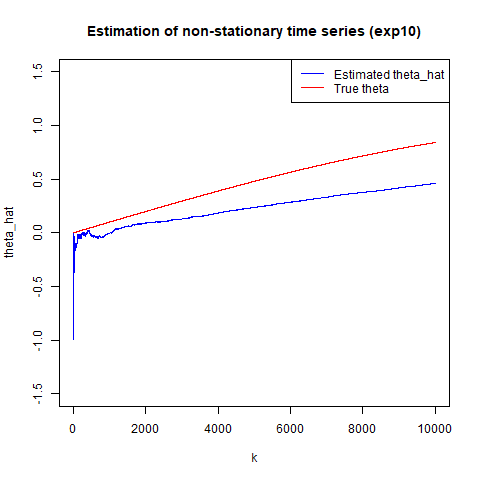
\includegraphics[width=.82\linewidth]{graphs/task10.png}
  \caption{忘却係数付きRLSによる非定常平均の追従($\gamma=0.99$)}
  \label{fig:task10}
\end{figure}

\paragraph{考察}
% 追従と平滑化のトレードオフ:$\gamma\downarrow$ で追従性↑ だが分散↑。$\gamma\uparrow$ で分散↓ だが遅延↑。
% 本設定は振幅1に対し雑音振幅1でSNRが低い。RMSEや相関係数で評価するとよい。
% スカラー回帰(φ_k=1)ではRLSは指数移動平均に近い挙動を示す。初期Φを大きくすると初期ゲインが大きく収束が速い。
